\documentclass{article}%
\usepackage[T1]{fontenc}%
\usepackage[utf8]{inputenc}%
\usepackage{lmodern}%
\usepackage{textcomp}%
\usepackage{lastpage}%
\usepackage{authblk}%
\usepackage{graphicx}%
%
\title{Physical characterisation of Tenacibaculum maritimum for vaccine development}%
\author{Debra Braun}%
\affil{Department of Cardiology, Zhongda Hospital, Medical School of Southeast University, Nanjing, Jiangsu, China}%
\date{01{-}01{-}1999}%
%
\begin{document}%
\normalsize%
\maketitle%
\section{Abstract}%
\label{sec:Abstract}%
SAN DIEGO {-} Researchers may finally gain the ability to sequence the DNA of long{-}dead civilizations to learn more about their biological and psychological background.\newline%
But there are still too many challenges ahead.\newline%
A team at Harvard University has produced the first, so far, blueprint that uses DNA to track individual genome activity in specific species.\newline%
The Harvard scientists expect the blueprint, known as a serological profile, to be useful in a variety of biological fields, from social engineering to genome mapping.\newline%
So far, four experiments have revealed that the distinctive "route genes" codes for have only eight regions where the genetic elements are as old as the species.\newline%
But this blueprint, done by preserving a region from the entire chromosome and comparing it to the sequence of the DNA map, offers clues about the genetic background of the species.\newline%
"We need to do work on the relatively small fragments of DNA and not to make a fancy map," said Robert Getman, head of the department of biological sciences at Harvard.\newline%
The researchers have taken these two narrow regions in the genome{-}{-}layering them slightly so there are two genetic branches that branch out of one another{-}{-}and printed them on such a small beam. The beam is composed of six tiny copies of each chromosome.\newline%
The arrays are injected into new bacteria, but at the same time they are mated with several types of sequence, like that that has been known in DNA that is repaired in culture.\newline%
"Eventually we hope the sequences will be able to be reprogrammed to improve the genes," Getman said.\newline%
"If these sequences can be reprogrammed to help other bacteria do the same things, we could use them to model how small organisms live, which could be used for evolution and disease."\newline%
Contact Surya Kumar at (202) 831{-}0404 or sarabaday.kumar@msn.com.

%
\subsection{Image Analysis}%
\label{subsec:ImageAnalysis}%


\begin{figure}[h!]%
\centering%
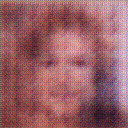
\includegraphics[width=150px]{500_fake_images/samples_5_262.png}%
\caption{A Man In A Suit And Tie Is Looking At The Camera}%
\end{figure}

%
\end{document}